\documentclass[11pt]{article}
\usepackage[margin=1in]{geometry}
\usepackage{amsmath}
\usepackage{amssymb}
\usepackage{xcolor}
\usepackage{tikz}

\title{Q3(d) 2023 Midterm: Hicksian Demand Explanation}
\author{ECO 310}
\date{}

\begin{document}

\maketitle

\section{The Question}

Harry's preferences are $u(N, C) = C^2 + 2CN$ (where $\alpha = 2$).

\textbf{Part (d)(ii):} Netflix and cable are free, but Harry has limited time. How much time $T$ does he need to achieve utility $u^*$?

\section{Why This Is a Hicksian/Expenditure Problem}

This question asks: \textit{``What's the minimum amount of time (expenditure) needed to achieve a target utility level $u^*$?''}

This is \textbf{exactly} the Hicksian demand problem from your study guide:

\begin{center}
\colorbox{yellow!30}{
\begin{minipage}{0.9\textwidth}
\textbf{Hicksian Problem:}
\[
\min_{x} \, p \cdot x \quad \text{subject to} \quad u(x) \geq \bar{u}
\]
\end{minipage}
}
\end{center}

In this specific question:
\begin{itemize}
    \item The ``expenditure'' is \textbf{time} $T = C + N$ (not money)
    \item The ``prices'' are both 1 (each hour of Netflix or Cable costs 1 hour of time)
    \item The constraint is achieving utility level $u^*$
\end{itemize}

\section{Step-by-Step Solution}

\subsection{Step 1: Set Up the Problem}

We want to minimize time expenditure:
\[
\min_{C, N} \, T = C + N
\]
subject to achieving the target utility:
\[
u(N, C) = C^2 + 2CN \geq u^*
\]

\subsection{Step 2: Find the Optimal Allocation (Tangency Condition)}

At the optimum, the marginal rate of substitution equals the price ratio:
\[
\frac{MU_C}{MU_N} = \frac{p_C}{p_N}
\]

Calculate the marginal utilities:
\begin{align*}
MU_C &= \frac{\partial u}{\partial C} = 2C + 2N \\
MU_N &= \frac{\partial u}{\partial N} = 2C
\end{align*}

Therefore:
\[
\frac{MU_C}{MU_N} = \frac{2C + 2N}{2C} = \frac{C + N}{C} = 1 + \frac{N}{C}
\]

Since both ``prices'' are 1 (one hour each):
\[
1 + \frac{N}{C} = \frac{p_C}{p_N} = \frac{1}{1} = 1
\]

This gives us:
\[
\frac{N}{C} = 0 \quad \Rightarrow \quad \boxed{N = 0}
\]

\subsection{Step 3: Find the Hicksian Demand}

Now we use the utility constraint. With $N = 0$:
\[
u^* = C^2 + 2C(0) = C^2
\]

Solving for $C$:
\[
\boxed{C = \sqrt{u^*}}
\]

This is the \textbf{Hicksian demand} for cable: $h_C(p_C=1, p_N=1, u^*) = \sqrt{u^*}$

And the Hicksian demand for Netflix is: $h_N(p_C=1, p_N=1, u^*) = 0$

\subsection{Step 4: Find the Expenditure Function}

The total time needed (expenditure function) is:
\[
\boxed{T = e(p_C=1, p_N=1, u^*) = C + N = \sqrt{u^*} + 0 = \sqrt{u^*} \text{ hours}}
\]

\section{Key Insights}

\subsection{Why Does Harry Choose Zero Netflix?}

When both goods have the same ``price'' (1 hour each), Harry compares their marginal utilities:
\begin{itemize}
    \item $MU_C = 2C + 2N$ (marginal utility of cable)
    \item $MU_N = 2C$ (marginal utility of Netflix)
\end{itemize}

Since $MU_C > MU_N$ whenever $N > 0$, cable gives more ``bang per buck'' (or bang per hour). So Harry specializes completely in cable.

\subsection{Connection to Marshallian Demand}

Compare this to part (c), which found the \textbf{Marshallian demand} (income $m$ is fixed):

\begin{center}
\begin{tabular}{|l|l|l|}
\hline
\textbf{Type} & \textbf{What's Fixed?} & \textbf{Question} \\
\hline
Marshallian (part c) & Income/budget $m$ & ``What should I buy with my budget?'' \\
Hicksian (part d) & Utility level $u^*$ & ``What's the cheapest way to get utility $u^*$?'' \\
\hline
\end{tabular}
\end{center}

\subsection{Graphical Interpretation}

\begin{center}
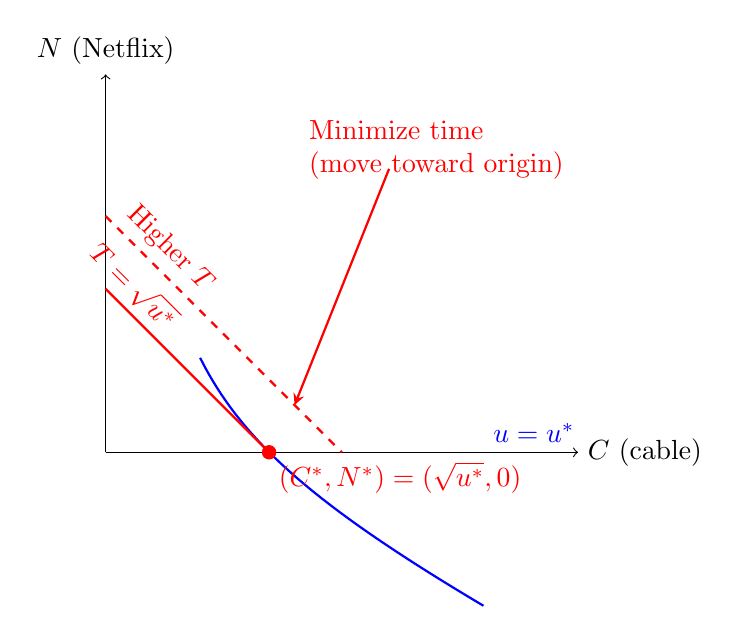
\begin{tikzpicture}[scale=1.2]
% Axes
\draw[->] (0,0) -- (5,0) node[right] {$C$ (cable)};
\draw[->] (0,0) -- (0,4) node[above] {$N$ (Netflix)};

% Indifference curve (hyperbola-like for this utility function)
\draw[thick, blue, domain=1:4, smooth, samples=100] plot (\x, {(3 - \x*\x)/(2*\x)});
\node[blue, right] at (4, 0.2) {$u = u^*$};

% Iso-cost lines (with slope -1 since both prices = 1)
\draw[thick, red, dashed] (0, 2.5) -- (2.5, 0);
\node[red, above left, rotate=-45] at (1, 1.5) {Higher $T$};

\draw[thick, red] (0, 1.73) -- (1.73, 0);
\node[red, above left, rotate=-45] at (0.6, 1.1) {$T = \sqrt{u^*}$};

% Optimal point
\filldraw[red] (1.73, 0) circle (2pt) node[below right] {$(C^*, N^*) = (\sqrt{u^*}, 0)$};

% Note the tangency occurs at N=0 (boundary solution)
\draw[thick, red, ->, >=stealth] (3, 3) -- (2, 0.5);
\node[red, align=left] at (3.5, 3.2) {Minimize time\\(move toward origin)};

\end{tikzpicture}
\end{center}

The Hicksian problem finds the point on the indifference curve $u = u^*$ that minimizes time expenditure $T = C + N$. The optimal point is $(\sqrt{u^*}, 0)$ on the horizontal axis.

\section{Summary}

Part (d)(ii) is a \textbf{Hicksian/expenditure minimization problem}:
\begin{enumerate}
    \item \textbf{Goal:} Minimize time expenditure to achieve utility $u^*$
    \item \textbf{Method:} Use tangency condition $\frac{MU_C}{MU_N} = \frac{p_C}{p_N}$ with constraint $u = u^*$
    \item \textbf{Result:} Hicksian demands are $h_C = \sqrt{u^*}$ and $h_N = 0$
    \item \textbf{Expenditure function:} $e(1, 1, u^*) = \sqrt{u^*}$ hours
\end{enumerate}

This contrasts with part (c), which solved the Marshallian problem: maximize utility given a fixed budget $m$.

\end{document}
